\documentclass[aspectratio=169,10pt]{beamer}

\usepackage[utf8]{inputenc}
\usepackage{amsmath}
\usepackage{booktabs}
\usepackage{graphicx}
\usepackage{array}

\graphicspath{{../results/}}

\definecolor{AskBlue}{RGB}{23,63,95}
\definecolor{AskGold}{RGB}{214,137,16}
\definecolor{AskSlate}{RGB}{70,78,92}

\usetheme{Madrid}
\usecolortheme{default}
\setbeamertemplate{navigation symbols}{}
\setbeamertemplate{footline}[frame number]

\setbeamercolor{title}{fg=white,bg=AskBlue}
\setbeamercolor{frametitle}{fg=white,bg=AskBlue}
\setbeamercolor{structure}{fg=AskBlue}
\setbeamercolor{block title}{fg=white,bg=AskBlue}
\setbeamercolor{block body}{fg=black,bg=black!3}
\setbeamercolor{normal text}{fg=black,bg=white}
\setbeamercolor{alerted text}{fg=AskGold}

\setbeamerfont{title}{series=\bfseries,size=\LARGE}
\setbeamerfont{frametitle}{series=\bfseries,size=\large}

\title{Ask or Act for Cooperative Assistance via Inverse Planning}
\subtitle{CS6208 Final Presentation}
\author[Zhu Yufan]{\texorpdfstring{Zhu Yufan \\ A0238993J}{Zhu Yufan (A0238993J)}}
\date{April 2026}

\begin{document}

\begin{frame}[plain]
  \titlepage
\end{frame}

\begin{frame}{Problem}
  \begin{columns}[T,onlytextwidth]
    \column{0.58\textwidth}
      \begin{itemize}
        \item A cooperative helper must choose between \alert{acting now} and \alert{asking a clarifying question}.
        \item Under ambiguous language and a hidden goal, acting too early risks the wrong object.
        \item Asking too often also has cost: it consumes time and can delay task completion.
      \end{itemize}
      \vspace{0.4em}
      \begin{block}{Goal}
        Learn a policy that asks \textbf{only when the expected value of information outweighs the cost}.
      \end{block}
    \column{0.38\textwidth}
      \begin{block}{Core question}
        When should a helper seek more information instead of committing to a likely goal?
      \end{block}
      \begin{itemize}
        \item Hidden principal goal
        \item Ambiguous instruction
        \item Noisy observed behavior
      \end{itemize}
  \end{columns}
\end{frame}

\begin{frame}{Task Setup}
  \begin{columns}[T,onlytextwidth]
    \column{0.45\textwidth}
      \begin{itemize}
        \item $9\times9$ two-room gridworld with 6 objects.
        \item Principal has a \textbf{hidden goal object} and gives an ambiguous instruction.
        \item Ambiguity level $K \in \{1,2,3,4\}$ is the number of candidate goals matching the instruction.
        \item Principal acts approximately rationally with Boltzmann parameters $\beta$ and $\varepsilon$.
        \item Assistant sees state, instruction, and principal motion, but not the true goal.
      \end{itemize}
    \column{0.55\textwidth}
      \centering
      
\includegraphics[width=\textwidth]{setup_overview.png}
  \end{columns}
\end{frame}

\begin{frame}{AskOrAct Method}
  \small
  \begin{itemize}
    \item Maintain a posterior over candidate goals from the instruction and inverse planning.
    \item Update the posterior after each observed principal action.
    \item Compare the expected team cost of acting now against asking the best available question.
  \end{itemize}
  \vspace{0.2em}
  \centering
  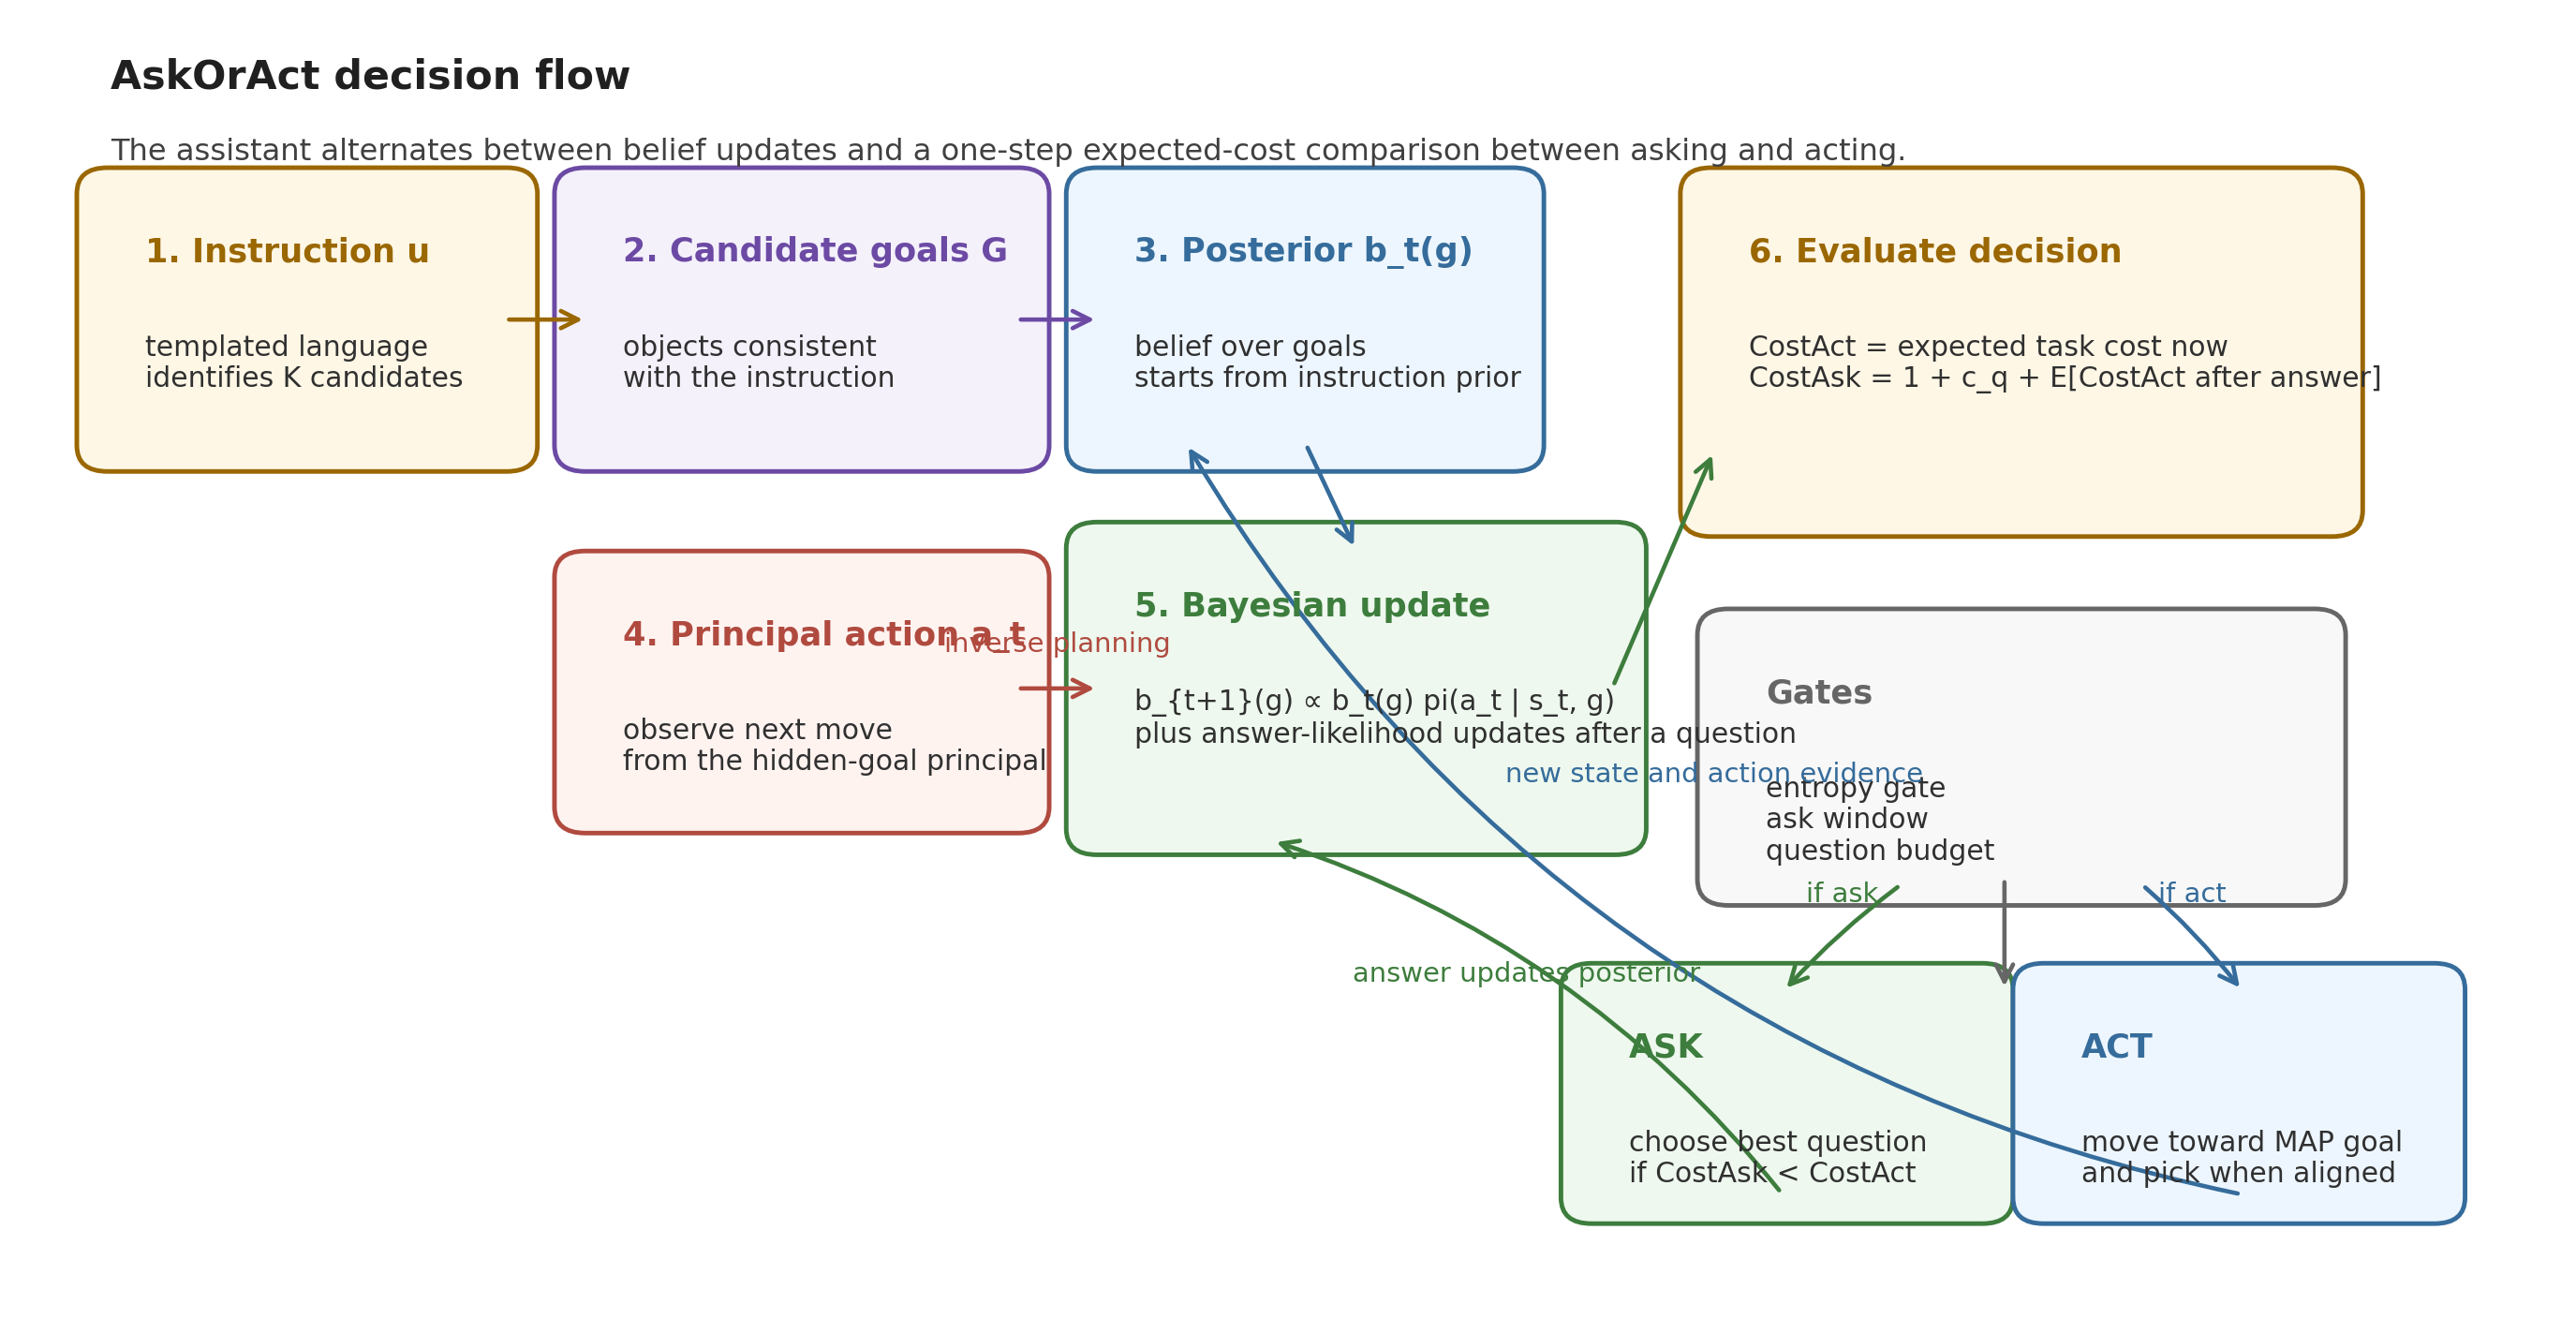
\includegraphics[width=0.76\textwidth]{ask_or_act_pipeline.png}
\end{frame}

\begin{frame}{Decision Rule and Baselines}
  \begin{columns}[T,onlytextwidth]
    \column{0.54\textwidth}
      \begin{block}{Ask-or-act comparison}
        \[
          \text{CostAct} = \sum_g b_t(g)\,\text{dist}(s_t,g)
        \]
        \[
          \text{CostAsk}(q) = 1 + 0.5 + \mathbb{E}_{\alpha}[\text{CostAct after answer } \alpha]
        \]
        Ask the best question only if it beats acting now.
      \end{block}
      \begin{itemize}
        \item Entropy gate: skip asking if already confident
        \item Ask window: no new questions after step 6
        \item Budget: at most 3 questions per episode
      \end{itemize}
    \column{0.43\textwidth}
      \small
      \begin{itemize}
        \item \textbf{AskOrAct}: ask only when VoI exceeds cost
        \item \textbf{NeverAsk}: act on MAP goal
        \item \textbf{AlwaysAsk}: ask until budget
        \item \textbf{InfoGainAsk}: gated highest-IG ask
        \item \textbf{EasyInfoGainAsk}: one-question IG
        \item \textbf{RandomAsk}: gated random ask
        \item \textbf{POMCPPlanner}: POMDP search at $K{=}2$
      \end{itemize}
  \end{columns}
\end{frame}

\begin{frame}{Evaluation Protocol}
  \begin{columns}[T,onlytextwidth]
    \column{0.58\textwidth}
      \begin{itemize}
        \item Sweep: $K \in \{1,2,3,4\}$, $\varepsilon \in \{0,0.05,0.1\}$, $\beta \in \{1,2,4\}$.
        \item 5 replicate seeds and 20 episodes per condition.
        \item 5 core policies evaluated in every cell.
        \item EasyInfoGainAsk and POMCPPlanner added as targeted stronger baselines at $K{=}2$.
      \end{itemize}
      \begin{block}{Metrics}
        Success rate, regret vs.\ oracle, questions per episode, and final MAP accuracy with 95\% bootstrap confidence intervals.
      \end{block}
    \column{0.36\textwidth}
      \begin{block}{Scale}
        \centering
        \Large 19,800 episodes
      \end{block}
      \begin{itemize}
        \item Reproducible seeds
        \item Dynamic deadlines
        \item Assistant-only completion
      \end{itemize}
  \end{columns}
\end{frame}

\begin{frame}{Main Results}
  \begin{columns}[T,onlytextwidth]
    \column{0.62\textwidth}
      \centering
      
\includegraphics[width=\textwidth]{main_dashboard.png}
    \column{0.34\textwidth}
      \begin{itemize}
        \item $K{=}1$: all policies collapse to the same easy case.
        \item $K{=}3$: AskOrAct beats NeverAsk by \textbf{+7.9 pp} success.
        \item $K{=}4$: AskOrAct beats NeverAsk by \textbf{+8.4 pp} success.
      \end{itemize}
      \begin{block}{Efficiency}
        AskOrAct reaches those gains while asking only about \textbf{0.6 questions per episode}.
      \end{block}
  \end{columns}
\end{frame}

\begin{frame}{Over-Asking vs Under-Asking}
  \begin{columns}[T,onlytextwidth]
    \column{0.53\textwidth}
      \small
      \begin{tabular}{lccc}
        \toprule
        Policy & Success & Regret & Q/ep \\
        \midrule
        InfoGainAsk & \textbf{91.7\%} & 2.88 & 1.31 \\
        \textbf{AskOrAct} & 87.3\% & \textbf{2.42} & 0.61 \\
        AlwaysAsk & 86.4\% & 4.56 & 2.58 \\
        NeverAsk & 78.9\% & 2.40 & 0.00 \\
        \bottomrule
      \end{tabular}
      \vspace{0.6em}
      \begin{block}{Interpretation at $K{=}4$}
        AskOrAct is the best balance point: it avoids NeverAsk's commitment errors and avoids AlwaysAsk's communication overhead.
      \end{block}
    \column{0.43\textwidth}
      \begin{itemize}
        \item AlwaysAsk uses about \textbf{4x} as many questions as AskOrAct.
        \item That extra questioning does \textbf{not} translate into better team cost.
        \item InfoGainAsk gets higher success, but pays for it in regret.
      \end{itemize}
  \end{columns}
\end{frame}

\begin{frame}{Pareto View}
  \begin{columns}[T,onlytextwidth]
    \column{0.60\textwidth}
      \centering
      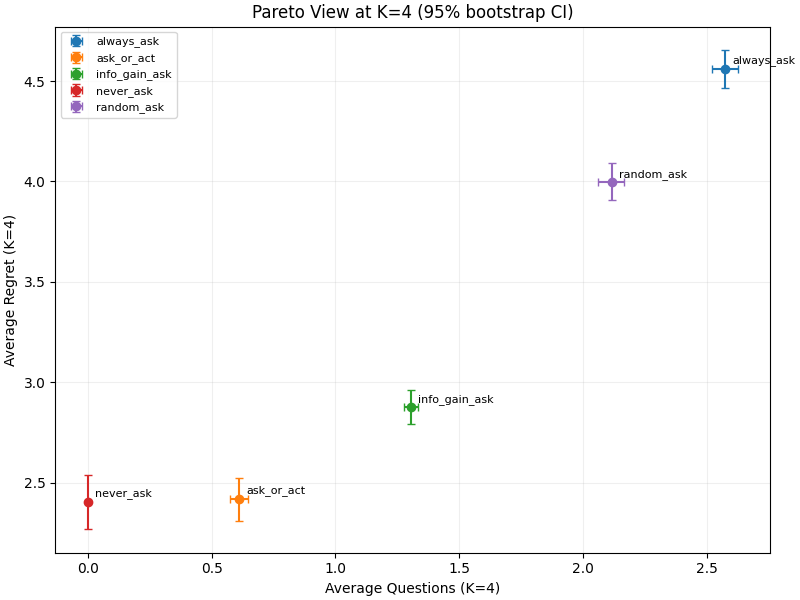
\includegraphics[width=\textwidth]{pareto_K4.png}
    \column{0.36\textwidth}
      \begin{itemize}
        \item AskOrAct is \textbf{Pareto-efficient} at high ambiguity.
        \item It dominates NeverAsk on success.
        \item It dominates AlwaysAsk and RandomAsk on regret.
        \item InfoGainAsk reaches higher success, but only by paying a higher coordination cost.
      \end{itemize}
  \end{columns}
\end{frame}

\begin{frame}{Robustness and Ablations}
  \begin{columns}[T,onlytextwidth]
    \column{0.58\textwidth}
      \centering
      
\includegraphics[width=\textwidth]{robust_mismatch_deltas.png}
    \column{0.39\textwidth}
      \begin{itemize}
        \item Under principal-model mismatch, AskOrAct still outperforms NeverAsk.
        \item Hardest case: true $\beta=1$ gives about \textbf{+13.5 pp} success over NeverAsk.
        \item Answer-noise sweeps and scale-$K$ tests preserve the same ordering.
      \end{itemize}
      \vspace{0.4em}
      \begin{block}{Ablation takeaway}
        A non-zero question cost is essential. Zero-cost asking leads to over-asking and lower success.
      \end{block}
  \end{columns}
\end{frame}

\begin{frame}{Takeaways}
  \begin{enumerate}
    \item \textbf{Selective asking works.} AskOrAct improves success by about 8 pp at $K{=}3,4$ with fewer than 1 question per episode.
    \item \textbf{Both extremes fail.} NeverAsk under-queries; AlwaysAsk over-queries and pays high regret.
    \item \textbf{Communication cost matters.} Without it, the policy over-asks and becomes less effective.
    \item \textbf{The pattern is robust.} The advantage survives answer noise, principal mismatch, and held-out template tests.
  \end{enumerate}
  \vspace{0.7em}
  \begin{block}{Next step}
    Extend the framework beyond templated questions and small exact-inference environments.
  \end{block}
\end{frame}

\begin{frame}{Backup: Evaluation Bug Found and Fixed}
  \begin{itemize}
    \item An early setting used \texttt{ENTROPY\_GATE = 0.8}, which prevented AskOrAct from asking at $K{=}2$.
    \item Reason: the uniform prior over two goals has entropy $\ln 2 \approx 0.69$, so the gate always fired.
    \item Fix: reduce the threshold to \texttt{0.3}.
    \item After the fix, AskOrAct at $K{=}2$ improves to \textbf{96.7\%} success vs.\ NeverAsk at \textbf{91.1\%}.
  \end{itemize}
  \vspace{0.6em}
  \begin{block}{Why keep this slide?}
    Careful debugging and consistency checks were part of the empirical contribution, not separate from it.
  \end{block}
\end{frame}

\end{document}
